\documentclass[tikz, border=4pt]{standalone}
\usepackage{tikz}
\usepackage{tikz-timing}
\begin{document}
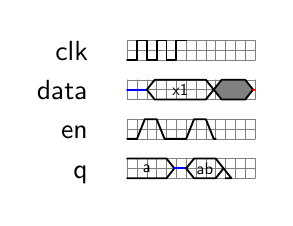
\begin{tikzpicture}[x=1cm, y=1cm]
  \node at (1.4,-0.96) {\pgfinterruptpicture%
  \begin{tikztimingtable}[timing/rowdist=2, timing/coldist=2, timing/slope=0.4]
    clk & 6{c} \\
    data & 2z 3D{x1} 2U 1x \\
    en & l 2h 3l 2h 1t \\
    q & 2D{a} 2z 3d{ab} 1l \\
  \extracode
    \tablegrid
  \end{tikztimingtable}%
  \endpgfinterruptpicture};
\end{tikzpicture}
\end{document}
